\documentclass[notitlepage,12pt]{article}
\usepackage{setspace}
\doublespacing

% Packages to use
\usepackage{graphicx}
\usepackage[table]{xcolor}
\usepackage{natbib}
\usepackage[margin=1in]{geometry}
\usepackage{fancyhdr}
\pagestyle{fancy}
\lhead{The Rise in Returns to Skill?}
\rhead{Senan Hogan-H.}

\usepackage{float}
\usepackage{hyperref}
\usepackage{amsmath}

% Author
\author{Senan Hogan-H.\footnote{This paper was completed in accordance with requirements for the Pomona College Department of Economics Senior Seminar, Spring 2018.  I am grateful for the comments and guidance of Michael Kuehlwein, Pomona College Department of Economics.} \\ Senior Seminar in Economics, Pomona College\footnote{\href{https://github.com/shoganhennessy/ECON190}{\color{blue}{\underline{This project's Github repository, which hosts all contributing materials, is available here.}}}}}

% Title
\title{The Rise in Returns to Skill? \\ \Large{A Modern Regression Analysis of Wage Inequality in the Current Population Survey (CPS)}}

% Date
\date{May 2018}
%%% BEGIN %%%
\begin{document}
\maketitle
\thispagestyle{empty}
% Abstract
\begin{abstract}
Abstract goes here.
\end{abstract}

\newpage
\setcounter{page}{1}

% Introduction
\section{Introduction}
Wage inequality has been documented as rising for many years in the economic literature, yet evidence that attributes this to a rise in return to skill use out-dated and orthodox regression approach to predicting wages.  Multiple significant studies decompose wage inequality in order to attribute a large portion of the rise in inequality to result from a rise in returns to skill, including most notably \cite{juhn1993wage}.

Narrative: how much of estimated wage inequality and corresponding rise in return to skill is due to (possibly naive) model choice?  

This paper: strip back the cumbersome assumptions and run with alternative models/frameworks.

How useful the Mincer wage equation is, with theoretical framework, and yet none of that is useful here.

The paper is structured as follows.  Section 2 surveys current literature on wage inequality and decomposing by regression approaches.  Section 3 describes a framework for expanding the regression approaches to this topic with specifications of the regression approaches used, both common-place and novel, as well as a description of the March CPS data set they are applied to.  Section 4 presents the empirical results of each approach.  Section 5 discusses the findings of the paper, with lessons to learn for studies that use predictive models and regression approaches in the study of wage inequality.

% LIT REVIEW
\section{Literature Review}
Wage inequality has increased dramatically since the 1950's in the US.  Many studies in labour economics attribute this this rise in inequality a rise in return to skill.  Across the other subfields of economics, however, there are multiple factors that also explain rising inequality, ranging from rise in market power \citep{furman2015firm}, to de-unionisation and supply and demand shocks \citep{DML95}, to ``skill-biased technological change'' \citep{acemoglu1998new,acemoglu2002technical}.  The literature that attributes a large percentage of the rise in wage inequality to an increase in returns to skill mainly relies on regression approaches pioneered by \cite{mincer1958investment,mincer1974schooling}.  Today, we have a greater repository of econometric and statistical methods to draw from in predicting wages and wage inequality by regression approaches.  These newer methods provide an avenue to better estimate the role of returns to skill in explaining rising wage inequality.

\cite{juhn1993wage} showed a drastic rise in wage inequality between 1963 and 1989, using the March CPS -- a representative data set for the US population.  The analysis extends the decomposition method of \cite{jmp2011} that focuses on the residuals in a standard regression to predict wages, interpreting wage inequality as the price of unobserved skills.  The methods make a few notable assumptions, notably primary choice of model to predict wages and that position in the income distribution is an accurate predictor for unobserved skill.  \cite{yun2009wage} questions the validity of using the change in distribution of residuals to explain discrimination in the decomposition methods of \cite{jmp2011,juhn1993wage}, while \cite{lemieux2006increasing} attributes the rise in wage inequality to a secular increase in experience and education, attributing the results of \cite{juhn1993wage} to composition factors and noisy data.

The Mincer wage equation was popularised in labour economics by \cite{mincer1958investment,mincer1974schooling}, where the standard Ordinary-Least-Squares (OLS) regression method is used to predict wages by simple function of potential experience and years of education.  This method was noted as being successful in explaining wages and wages inequality while maintaining an intuitive basis, and has become a benchmark model in labour economics as a result.  \cite{juhn1993wage} use this approach to predict wages, crucially using the fact that the method produces much worse estimates (i.e. higher errors) in the late 1980's that did in earlier decades.  However, today the Mincer wage equation is noted as in need of adjustments to capture changes in the US economy and acknowledge advances in empirical labour economics.  \cite{lemieux2006mincer} specifically proposes functional adjustments to accommodate changes in the economic relationship between years of education and wages seen in wage data until the 1990's.  However, the US economy is very different to how it was in the 1950's, especially in terms of size, complexity and technology.  Today, supply chains are increasingly complicated and dependent on global markets, entire industries have risen and fallen with ramifications for structural employment, and the Internet has revolutionised many sectors of the economy.  Labour economic studies that use the original Mincer wage function to predict wages in the modern economy do not fully acknowledge the rise in complexity or resulting changes in the determinants of wages,\footnote{That is the simple linear equation may only capture changes through an increase in estimated returns to education, experience and potential experience, yet may not acknowledge any change in the composition or functional form of them and other important variables in determining wages.} and would do better to take advantage of advances in regression methods that can better accommodate.\footnote{More advanced regression practices will also have the advantage of predicting wages without onerous assumptions in the underlying data and economy, as in \cite{juhn1993wage}.} 

Regression practices have advanced tremendously in the last few decades, and since Dr Jacob Mincer began modern labour economics as a field.  The original Mincer wage equation does provide a method for intuitive prediction of wages, though an overly simplified version of the story.  There are many variables -- observed, unobserved, or even unobservable -- with possible explanatory power for wages in the US economy.  There are also many ways in which these variables explain wages (linear or non-linear), and certainly in different ways to how they did in previous decades.  This problem is not be completely fixed by a simple adjustment, as noted by \cite{lemieux2006increasing}.  These issues bring in to question the robustness of only using simple OLS approach in analyses that require prediction of wages with given data.

Regression by machine learning practices provide a viable avenue to expand the literature, and more robustly estimate returns to skill in the US economy.  A regression tree is a completely different form of regression than OLS and other common econometric methods.  The process involves building a decision tree by minimising an error function, allowing any level of non-linearities in model estimation.  Bootstrapping of data used to form the model forms a random forest model, with extremely high power for prediction with less problems of over-fitting data \citep{breiman2001random}.  Labour economics  has so far been slow to use such techniques in empirical studies.  \cite{belloni2011high} and \cite{abadie2017risk} develop novel prediction techniques, and example their properties by predicting wages in the March CPS.  Importantly, \cite{chalfin2016productivity} demonstrate the benefit of predictive power of tree-based machine learning methods in productivity of public sector workers.  Gains in predictive power from these methods are noted as ``large both absolutely and relative to those from interventions studied by standard causal analyses in microeconomics.''  Lastly, the March CPS is an extremely large data set, especially when treated in 5 year increments,\footnote{See Section 3.1 for an expanded discussion of this issue.} and so provides an adequate place to use newer regression practices as outlined by \cite{varian2014big}.

This paper applies multiple regression-based predictive models -- including the novel random forest method -- to a representative data set of the United States, suitably large for big-data practices.  The results are presented in the wider context of previous research on the rising returns to skill, and the role of using newer regression and big-data practices in the field of labour economics.


\section{Wage Inequality in the US}

Explain the issue and history in the US.  Explain acceleration for 1980 and beyond.  Provide some graphs.

\subsection{Data}
The analysis of this paper is conducted on 27 years of wage and demographic information for individuals taken from the March the Annual Social and Economic Supplement of the Current Population Survey, commonly referred to as the March CPS.  The 27 years refer to 1980--2016 (inclusive), with data referring to the 12 months preceding the March survey.  Uniform extracts of the March CPS are taken, in full, from publicly available hosting by the Centre for Economic Policy Research \nocite{center} (Version 1.0, 2016).

Analysis of inequality refers to wage information at the hourly level, defined as annual earnings divided by annual hours worked,\footnote{Weekly hours worked times by amount of weeks worked in a year.} and annual level, defined as total income in the 12 months preceding, as specified.  Wages are adjusted according to the CPI Research Series Using Current Methods (CPI-U-RS), set to 2015 dollars.\footnote{These specifications for wages are provided in full by the CEPR Extracts.}  The sample is restricted to a sample meant to be representative of full-time workers, both male and female.\footnote{Whereas \cite{juhn1993wage} analyse only men's wages in order to remove effects of rising women's labour force participation.  This study however considers a later time period when women participation is relatively similar and so includes women.}  Only full-time employed workers are included, making at least the 2015 hourly federal minimum wage (\$7.25), positive total annual income, and between the ages 18 and 65.  See Table 1 for summary statistics for real hourly and annual wage, age, years of education, and proportion female for the sample.

\begin{table}[!htbp] \centering 
  \caption{Summary Statistics, 1980-2016} 
  \label{} 
\begin{tabular}{@{\extracolsep{5pt}}lccccc} 
\\[-1.8ex]\hline 
\hline \\[-1.8ex] 
Statistic & \multicolumn{1}{c}{No. Observations} & \multicolumn{1}{c}{Mean} & \multicolumn{1}{c}{St. Dev.} & \multicolumn{1}{c}{Min} & \multicolumn{1}{c}{Max} \\ 
\hline \\[-1.8ex] 
Hourly Wage, \$ & 2,199,241 & 25.38 & 334.70 & 7.25 & 444,241.80 \\ 
Annual Income, \$ & 2,199,241 & 50,487.30 & 51,064.77 & 4,060.05 & 1,848,079.00 \\ 
Age & 2,199,241 & 39.63 & 11.67 & 18 & 65 \\ 
Years of Education & 2,199,241 & 13.72 & 2.74 & 0 & 22 \\ 
Female & 2,199,241 & 0.460 & 0.498 & 0 & 1 \\ 
\hline \\[-1.8ex] 
\end{tabular} 
\end{table}

\subsection{Rising Inequality}

Some graphs

\section{Explaining Wage Inequality}

Wage Inequality has risen significantly since 1980, and for years preceding.  The role of changing returns to skills, observable or unobservable, plays in explaining this rising in inequality is not quite so clearly cut.  Equation 1 presents a standard linear regression that aims to decompose wage inequality in the form of a standard wage equation. 
\begin{equation}
Y_{it} = \mathbf{X}_{it}\beta_t + \varepsilon_{it}
\end{equation}
$Y_{it}$ represents the log weekly wage for individual $i$ in year $t$, $\mathbf{X}_{it}$ a vector of observable characteristics and $\beta_t$ the vector of coefficients representing returns to observable skills. $\varepsilon_{it}$ is the standard residual, the component for wages that are not otherwise explained by specified variables in the given regression method (unobserved characteristics).  This residual may be specified in terms of position of the income distribution, in equation 2, where $F_{it}(. | \mathbf{X}_{it})$ is the cumulative density function for individuals with observed characteristics $\mathbf{X}_{it}$ in year $t$.
\begin{equation}
\varepsilon_{it} = F_{t}^{-1}(\theta_{it} | \mathbf{X}_{it})
\end{equation}

\cite{juhn1993wage} present this framework for predicting wages, with slight adjustments to specify whether returns to observable skill may be vary year on year, and a fixed distribution (across all years) for the residuals.  

\subsection{Prediction Methods}
The residual, $\varepsilon_{it}$, and its distribution is crucial in these methods to document the rise in returns to unobservable skill.  It follows that the methods used to generate the residuals and the way that ``unobserved'' skills are defined dramatically influence their estimated returns.
An important choice to be made is the choice of regression method and form that equation 1, section 5 takes.

\subsubsection{Mincer Wage Equation}
The vast majority of labour economics studies that decompose wages use the Mincer wage equation to predict wages.  The approach applies Ordinary Least Squares regression algorithm to the Mincer earnings function, which dates back to some of the first labour economics studies that focus on wage inequality in \cite{mincer1958investment, mincer1974schooling}.  The function to be estimated by this approach takes the following form.
\begin{equation}
Y_{it}  = Y_0 + \rho s_{it} +\beta_1 x_{it} + \beta_2 x_{it}^2 + \varepsilon_{it}
\end{equation}
Here, $Y_{it}$ represents the log wage for individual $i$ in year $t$, $s_i$ years of education, and $Y_0$ the standard intercept, $\rho$, $\beta_1$, $\beta_2$ standard coefficients to be estimated with error term $\varepsilon_{it}$.  Potential experience, $x_{it}$, is defined as age minus years of education -- 6, i.e. $x_{it} = Age_{it} - s_{it} - 6$.  This model is extremely influential in labour economics to describe and predict inequality in wages in the US population.  Its influence comes in part from its theoretical foundations and simplicity in interpretation, yet is documented as being only accurate in predicting wages for the 1950s. 

\subsubsection{Mincer Wage Equation, Adjusted}
\cite{lemieux2006mincer} proposes that the Mincer wage equation is expanded to take an expanded form.  The form is presented in equation 4, where the quadratic form for potential experience is expanded to a quartic, and a the years of education include a quadratic. 
\begin{equation}
Y_{it}  = Y_0 + \rho_{1t} s_{it} + \rho_{2t} s_{it}^2 + \beta_{1t} x_{it} + \beta_{2t} x_{it}^2 + \beta_{3t} x_{it}^3 + \beta_{4t} x_{it}^4 + \varepsilon_{it}
\end{equation}
The given variables are represented as in equation 3.  This functional form better captures advances in the economy, and so is noted as better predicting ages for later decades following the 1950's than the original form.  However, the returns to observable characteristics (i.e. estimated coefficients) are harder to interpret from an economic or intuitive point of view.  This form is also noted as accounting for cohort effects, by allowing estimates for coefficients to vary by time period.\footnote{Estimations by these methods note where the coefficients are allowed to vary by single years or a five year grouping.}

This adjusted form of the Mincer wage equation is used to predict wages while maintaining the standard OLS approach.  A local linear regression produces residual estimates, in addition, in order to compare a very similar approach that relaxes the assumptions associated with the linear parameter estimation in the OLS approach.

\subsubsection{Tree-Based Methods}

Tree-based methods are a more modern approach to regression and prediction.  The process involves building a tree in the following process.  A data set of interest is split in to a training sample and test sample.  The training sample is used to train the model, where an error function is minimised (similar to the OLS framework) for a defined amount of decisions.  The decisions take the form of a true-false condition on given variables, leading to a final prediction conditional on all the given conditions.  Figure 1 presents a decision tree to depict such a model for log wages 1980-1985, Figure 2 for 2010-2016.  [THIS PART IS UNDER WORK, GRAPHICS NEED EDITING]  The regression tree approach allows for non-linearities and interactions between variables. 
\begin{figure}[H]
  \centering
  \caption{Decision tree for real log wages, 1980-1985.}
  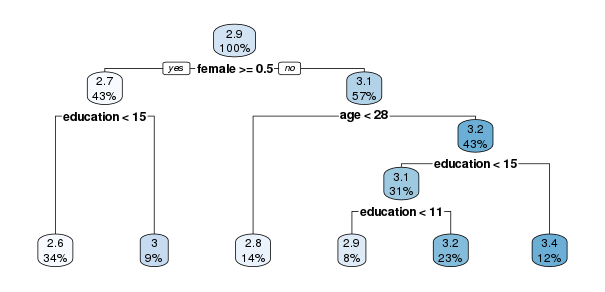
\includegraphics[width=4in, height=5cm]{Rpat1980_1985.pdf}
\end{figure}

\begin{figure}[H]
  \centering
  \caption{Decision tree for real log wages, 2010-2016.}
  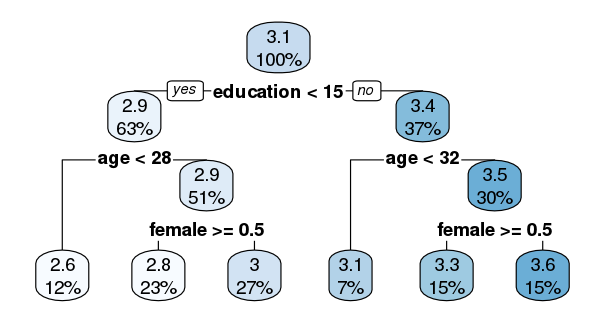
\includegraphics[width=6.5in, height=8cm]{Rpat2010_2016.pdf}
\end{figure}

The decision tree method often over-fits for the data set which it is built on, making for a model which is not generalisable for the entire population.  A random forest approach builds many, many trees based on bootstrapped samples of the entire data set and cross-validating across the sample,\footnote{Cross validation is a methods to chose best value of parameter in cost function minimisation, a technical detail in building the prediction model.} making for a model which is less likely to over-fit the training data set.  The approach makes a model extremely good at capturing non-linearities and interactions in given data, to process an method extremely good at predicting a response variable.

The variables selected in these models, of course, will be only those reasoned to be economically significant, taking note of points raised by \cite{mullainathan2017machine}.  The variable importance -- a very well defined concept in this machine learning approach -- will also be documented year on year, going on to assess returns to skill across time by importance of years of education in this model. 

\subsection{Residuals in Wage Inequality}
The above methods produce estimates for residuals in wage inequality, $\hat{\varepsilon}_{it}$, which will vary across methods of regression.  The distribution of the residuals represent returns to unobserved skills, according to \cite{juhn1993wage}.  The distribution of residuals of wage is noted as varying across the income distribution.  To demonstrate this point, a standard OLS regression in equation  5 shows present a linear estimate for how the residuals vary across the distribution.
\begin{equation}
\varepsilon_{it} = \varepsilon_{0} + \psi_t \theta_{it} + u_{it}
\end{equation}
Again, $\theta_{it}$ represents position in the income distribution (measured by a bin for a rank), so that the parameter to be estimated, $\psi$, represents how returns to unobserved skill vary linearly across the income distribution.


% RESULTS
\section{Results}

% DISCUSSION
\section{Discussion}

\subsection{Limitations}

Mention wage inequality vs inequality in general.  What about wealth and/or political inequality?

% Conclusion
\section{Conclusion}

\bibliographystyle{agsm}
\bibliography{bibliography}

\end{document}
